\documentclass{article}
%-------------------------------------------------------------------------------------------
\usepackage[pdftex,colorlinks,linkcolor=blue]{hyperref}
%-------------------------------------------------------------------------------------------
\usepackage{graphicx}
%-------------------------------------------------------------------------------------------
\begin{document}
\title{Velvet Manual - version 1.1}
\author{Daniel Zerbino}
\date{August 29, 2008}

%-------------------------------------------------------------------------------------------

\maketitle

\tableofcontents

\newpage

\section{For impatient people}

\begin{verbatim}
> make
> ./velveth
> ./velvetg

> ./velveth sillyDirectory 21 -shortPaired data/test_reads.fa
> ./velvetg sillyDirectory
	(Final graph has 16 nodes and n50 of 24184, max 44966, total 100080, 
	using 0/142858 reads)
> less sillyDirectory/stats.txt

> ./velvetg sillyDirectory -cov_cutoff 5 -read_trkg yes -amos_file yes
	(Final graph has 1 nodes and n50 of 99975, max 99975, total 99975, 
	using 135862/142858 reads)
> less sillyDirectory/velvet_asm.afg

> ./velvetg sillyDirectory -cov_cutoff auto
	(Final graph has 1 nodes and n50 of 99975, max 99975, total 99975, 
	using 0/142858 reads)

> ./velvetg sillyDirectory -exp_cov 19 -ins_length 100
	(Final graph has 12 nodes and n50 of 99975, max 99975, total 100165, 
	using 135855/142858 reads)
	
> ./velvetg sillyDirectory -exp_cov auto
	(Final graph has 1 nodes and n50 of 99975, max 99975, total 99975, 
	using 135862/142858 reads)

> ./velveth sillyDirectory 21 -short data/test_reads.fa -long data/test_long.fa
> ./velvetg sillyDirectory -exp_cov 19
	(Final graph has 10 nodes and n50 of 80927, max 80927, total 100122, 
	using 137863/144858 reads)
	
> ./velvetg sillyDirectory -exp_cov auto
	(Final graph has 1 nodes and n50 of 99975, max 99975, total 99975, 
	using 137862/144858 reads)

\end{verbatim}

\section{Installation}

\subsection{Requirements}

	Velvet should function on any standard 64bit Linux environment with
gcc. A good amount of physical memory (12GB to start with, more is no luxury)
is recommended. 
	
	It can in theory function on a 32bit environment, but such systems have memory limitations which might ultimately be a constraint for assembly.

\subsection{Compiling instructions}

\label{sec:compilation}

From a GNU environment, simply type:

\begin{verbatim}
> make
\end{verbatim}

\subsection{Compilation settings}

\subsubsection{Colorspace Velvet}

To produce the colorspace version of Velvet, compile with the instruction:

\begin{verbatim}
> make color
\end{verbatim}

All the rest of the manual remains valid, except that the executables are now called velveth\_de and velveth\_de . 

\textbf{Beware} that color- and sequence space are incompatible, hence separate sets of executables. In other words, don't try to hash sequence files with colorspace velvet or vice-versa, under penalty of meaningless results!

\subsubsection{CATEGORIES}

Because of the use of fixed-length arrays, a number of variables have to be set at compilation time. 

One of the is the number of channels, or categories of reads, which can be handled independently. This is for example useful is you want to distinguish reads from different insert libraries, or from different samples altogether.

By default, there are only two short read categories, but this variable can be extended to your needs. For example, to obtain 57 different channels, compile with the parameter:

\begin{verbatim}
make 'CATEGORIES=57'
\end{verbatim}

(Note the single quotes and absence of spacing.)

Obviously, the greater the number, the longer the corresponding arrays, the more memory will be required to run Velvet. Adjust this variable according to your needs and your memory requirements. 

\subsubsection{MAXKMERLENGTH.}

\label{sec:maxlength}

Another useful compilation parameter is the MAXKMERLENGTH. As explained in \ref{sec:kmercov}, the hash length can be crucial to getting optimal assemblies. Depending on the dataset, you might wish to use long hash lengths. 

By default, hash-lengths are limited to 31bp, but you can push up this limit by adjusting the MAXKMERLENGTH parameter at compilation time:

\begin{verbatim}
make 'MAXKMERLENGTH=57'
\end{verbatim}

(Note the single quotes and absence of spacing.)

By storing longer words, Velvet will be requiring more memory, so adjust this variable according to your needs and memory resources. 

\subsubsection{BIGASSEMBLY}

Read IDs are stored on signed 32bit integers, meaning that if you have a big assembly with more than 2.2 billion reads more memory is needed to track the reads. To do so, simply add the following option to the make command:

\begin{verbatim}
make 'BIGASSEMBLY=1'
\end{verbatim}

(Note the single quotes and absence of spacing.)

This will cost more memory overhead. 

\subsubsection{LONGSEQUENCES}

Read lengths are stored on signed 16bit integers, meaning that if you are assembling contigs longer than 32kb long, then more memory is required to store coordinates. To do so, simply add the following option to the make command: 

\begin{verbatim}
make 'LONGSEQUENCES=1'
\end{verbatim}

(Note the single quotes and absence of spacing.)

This will cost more memory overhead. 

\subsubsection{OPENMP}

To turn on multithreading, simply use the OPENMP option at compilation. This should not significantly affect the memory overhead or results: 

\begin{verbatim}
make 'OPENMP=1'
\end{verbatim}

OpenMP allows a program to make use of multiple CPU cores on the same machine. You might have to set the environment variables OMP\_NUM\_THREADS and OMP\_THREAD\_LIMIT. Velvet will the use up to $OMP\_NUM\_THREADS + 1$ or $OMP\_THREAD\_LIMIT$ threads. More information at \\
\href{ http://www.ats.ucla.edu/clusters/common/computing/parallel/using_openmp.htm}{http://www.ats.ucla.edu/clusters/common/computing/parallel/using\_openmp.htm}

Only parts of the Velvet algorithm make use of OpenMP, so don't expect a linear increase in run time with respect to CPUs.

\subsubsection{BUNDLEDZLIB}

By default, Velvet uses an existing zlib installed on your system. If there isn't one or if it is unsuitable for any reason, zlib source code is also distributed within the Velvet source package and Velvet can be compiled to use this bundled zlib by adding the following option to the make command:

\begin{verbatim}
make 'BUNDLEDZLIB=1'
\end{verbatim}

\section{Running instructions}

\subsection{Running velveth}

Velveth helps you construct the dataset for the following program, velvetg, and indicate to the system what  each sequence file represents.

If, on the command line, you forget the syntax, you can print out a short help message:
\begin{verbatim}
> ./velveth
\end{verbatim}

\label{sec:hashing}

Velveth takes in a number of sequence files, produces a hashtable, then outputs two files in an output directory (creating it if necessary), Sequences and Roadmaps, which are necessary to velvetg. The syntax is as follows:

\begin{verbatim}
> ./velveth output_directory hash_length 
            [[-file_format][-read_type] filename]
\end{verbatim}

The hash length, also known as $k$-mer length, corresponds to the length, in base pairs, of the words being hashed. See \ref{sec:kmercov} for a detailed explanation of how to choose the hash length.

\underline{Supported file formats are:}
\begin{description}
\item[fasta] (default) 
\item[fastq]
\item[fasta.gz]
\item[fastq.gz]
\item[sam]
\item[bam]
\item[eland]
\item[gerald]
\end{description}

\underline{Read categories are:}
\begin{description}
\item[short] (default)
\item[shortPaired]
\item[short2] (same as short, but for a separate insert-size library)
\item[shortPaired2] (see above) 
\item[long] (for Sanger, 454 or even reference sequences)
\item[longPaired]
\end{description}

For concision, options are stable. In other words, they are true until
contradicted by another operator. This allows you to write as many filenames
as you wish without having to re-type identical descriptors.  For example:
\begin{verbatim}
> ./velveth output_directory/ 21 -fasta -short solexa1.fa solexa2.fa solexa3.fa -long
capillary.fa
\end{verbatim}

In this example, all the files are considered to be in FASTA format,
only the read category changes. However, the default options are ``fasta'' and ``short'', so the previous example
can also be written as:

\begin{verbatim}
> ./velveth output_directory/ 21 solexa*.fa -long capillary.fa
\end{verbatim}

\subsubsection{Piping Velvet}

If you wish to run velveth directly on the output of another program, without the cost of creating and reading a new sequence file, then you can pipe it. In that case the character `-' is used to represent the standard input within the command line. 

Therefore, instead of having:

\begin{verbatim}
> myprogram > selected_reads.fa
> velveth directory 21 -fastq other_reads.fastq -fasta selected_reads
> velvetg directory (... parameters...) 
\end{verbatim}

You can simply do:

\begin{verbatim}
> myprogram | velveth directory 21 -fastq other_reads.fastq -fasta -
> velvetg directory (... parameters...) 
\end{verbatim}

\subsubsection{Strand specific sequencing}

If you are using a strand specific transcriptome sequencing protocol, you may wish to use this option for better results. Even though it can be used anywhere on the command line, it applies to all the dataset. To toggle it on, type:

\begin{verbatim}
> ./velveth output_directory/ 21 (...data files...) -strand_specific
\end{verbatim}

\subsubsection{Multiple k-mers}

If you wish for Velvet to efficiently test various k-mer lengths without doing redundant computations, you can request all k-mer lengths such that $m \le k \le M$ with a step of s:

\begin{verbatim}
> ./velveth output_directory/ m,M,s (..data files..)
\end{verbatim}

\subsubsection{Preprocessing the Sequences file}

It can often be interesting to pre-process the Sequences file before running the hashing. During this phase, Velvet simply reads the input files and prepares a file which contains them all. This can be done on a very small computer, thus not wasting cycles on a powerful computer. To do so, simply invoke the -noHash option:

\begin{verbatim}
> ./velveth output_directory/ 21 (..data files..) -noHash
\end{verbatim}

Once the Sequences file is prepared you can run velveth on the same directory, or any directory which contains a link to the same file (or a copy of that file if necessary):

\begin{verbatim}
> ./velveth output_directory/ 21 -reuse_Sequences
\end{verbatim}

\subsection{Running velvetg}

Velvetg is the core of Velvet where the de Bruijn graph is built then manipulated. Note that although velvetg saves some files during the process to avoid useless recalculations, the parameters are \textbf{not} saved from one run to the next. Therefore:

\begin{verbatim}
> ./velvetg output_directory/ -cov_cutoff 4
> ./velvetg output_directory/ -min_contig_lgth 100
\end{verbatim}

\ldots is different from:

\begin{verbatim}
> ./velvetg output_directory/ -cov_cutoff 4 -min_contig_lgth 100
\end{verbatim}

This means you can freely play around with parameters, without re-doing most of the calculations:

\begin{verbatim}
> ./velvetg output_directory/ -cov_cutoff 4
> ./velvetg output_directory/ -cov_cutoff 3.8
> ./velvetg output_directory/ -cov_cutoff 7
> ./velvetg output_directory/ -cov_cutoff 10
> ./velvetg output_directory/ -cov_cutoff 2
\end{verbatim}

On the other hand, within a single velvetg command, the order of parameters is not important.

Finally, if you have any doubt at the command line, you can obtain a short help message by typing:

\begin{verbatim}
> ./velvetg
\end{verbatim}

	\subsubsection{Single reads}
	
	\label{sec:velvetg}

Initally, you simply run: 
\begin{verbatim}
> ./velvetg output_directory/
\end{verbatim}

This will produce a fasta file of contigs and output some statistics.
Experience shows that there are many short, low-coverage nodes left over from the intial correction. Determine as you wish a coverage cutoff value (cf. \ref{sec:covcutoff}), say 5.2x, then type:

\begin{verbatim}
> ./velvetg output_directory/ -cov_cutoff 5.2
\end{verbatim}

On the other hand, if you want to exclude highly covered data from your assembly (e.g. plasmid, mitochondrial, and chloroplast sequences) you can use a maximum coverage cutoff:

\begin{verbatim}
> ./velvetg output_directory/ -max_coverage 300 (... other parameters ...)
\end{verbatim}

The coverage cutoff can also be set automatically to half the length weighted median contig coverage depth. Although you may wish to optimise this parameter in further iterations, this option allows you to quickly obtain a decent assembly in your first run. To do so, type:

\begin{verbatim}
> ./velvetg output_directory/ -cov_cutoff auto
\end{verbatim}

Note that typing $-exp\_cov$ $auto$ (cf. next subsection) is equivalent to typing $-exp\_cov$ $auto$ $-cov\_cutoff$ $auto$, unless you decide to manually set the coverage cutoff. On the contrary, $-cov\_cutoff$ $auto$ does not affect the expected coverage setting.

	\subsubsection{Adding long reads}
	
\textbf{Reminder:} you must have flagged your long reads as such when running
velveth (cf. \ref{sec:hashing}).
	
If you have a sufficient coverage of short reads, and any quantity of long reads (obviously the deeper the coverage and the longer the reads, the better), you can use the long reads to resolve repeats in a greedy fashion. 

To do this, Velvet needs to have a reasonable estimate of the expected coverage \emph{in short reads} of unique sequence (see \ref{sec:kmercov} for a definition of k-mer coverage). The simplest way to obtain this value is simply to observe the distribution of contig coverages (as described in \ref{sec:expcov}), and see around which value the coverages of nodes seem to cluster (especially the longer nodes in your dataset). Supposing the expected coverage is 19x, them you indicate it with the $exp\_cov$ marker:

\begin{verbatim}
> ./velvetg output_directory/ -exp_cov 19 (... other parameters ...)
\end{verbatim}

If you have reasons to believe that the coverage is reasonably uniform over your sample, you can request that Velvet estimate it for you, by typing:

\begin{verbatim}
> ./velvetg output_directory/ -exp_cov auto (... other parameters ...)
\end{verbatim}

This will set $exp\_cov$ to the length weighted median contig coverage, and $cov\_cutoff$ to half that value (unless you override it with a manual setting).

\textbf{Caveat emptor:} if this option is used on datasets with very heterogeneous coverage (e.g. transcriptomes, ChIP-seq, etc) then the results are simply unpredictable, and mis-assemblies are to be expected. This option is intended mainly for standard genomic sequencing.

	\subsubsection{Paired-ends reads}

\textbf{Reminder:} you must have flagged your reads as being paired-ends when running
velveth (cf. \ref{sec:hashing}).

To activate the use of read pairs, you must specify two parameters: the \emph{expected} (i.e. average) insert length (or at least a rough estimate), and the expected \emph{short-read k-mer coverage} (see \ref{sec:kmercov} for more information). The insert length is understood to be the length of the sequenced fragment, i.e. it includes the length of the reads themselves. If you expect your insert length to be around 400bp, and your coverage to be around 21.3x, you would type:

\begin{verbatim}
> ./velvetg output_directory/ -ins_length 400 -exp_cov 21.3 
	          (... other parameters ...)
\end{verbatim}

If one of the libraries is a mate-pair library made by circularization, and you have reasons to suspect the presence of read pair contamination, then you can flag that library to velvetg:

\begin{verbatim}
> ./velvetg output_directory/ -shortMatePair yes 
	          (... other parameters ...)
\end{verbatim}

If you happen to have hashed paired long reads and you ordered them as explained in \ref{sec:pairedformat} you can also tell Velvet to use this information for scaffolding by indicating the corresponding insert length (remember that you still need to indicate the short-read k-mer coverage):

\begin{verbatim}
> ./velvetg output_directory/ -exp_cov 21 -ins_length_long 40000 
		 (... other parameters ...)
\end{verbatim}

As with long reads, if you have reasons to believe that the coverage is reasonably uniform over your sample, you can request that Velvet estimate it for you, by typing:

\begin{verbatim}
> ./velvetg output_directory/ -exp_cov auto (... other parameters ...)
\end{verbatim}

This will set $exp\_cov$ to the length weighted median contig coverage, and $cov\_cutoff$ to half that value (unless you override it with a manual setting).

\textbf{Caveat emptor:} if this option is used on datasets with very heterogeneous coverage (e.g. transcriptomes, ChIP-seq, etc) then the results are simply unpredictable, and mis-assemblies are to be expected. This option is intended mainly for standard genomic sequencing.

\textbf{Automatically measuring the insert length} 

If the insert length of a library is unspecified, Velvet will attempt to measure it for you, based on the read-pairs which happen to map onto a common node. The corresponding $ins\_length*$ and $ins_length*\_sd$ parameters are thus set for you. This option is designed as a convenience if your assembly is initially good enough to provide long contigs to bootstrap the process. If that is not the case, the library insert length will be determined from a small sample size, and is liable to produce a poor estimate. You should check the Velvet console output to make sure the insert length estimates are not absurd.

\textbf{Scaffolding} By default, Velvet will try to scaffold contigs that it cannot quite connect. This results in sequences of \emph{N}s in the contigs.fa file, which correspond to the estimated distance between two neighbouring contigs. If you do not want this scaffolding, you can turn it off with the following switch:

\begin{verbatim}
> ./velvetg output_directory/ -exp_cov 21 -ins_length_long 200
		-scaffolding no (... other parameters ...)
\end{verbatim}

\textbf{Standard deviations} This is a more subtle point which you can ignore if you have only one dataset of paired-end reads or if the standard deviation (SD) of the insert lengths is roughly proportional to the expected length (e.g. if the insert-lengths are described as $length \pm p\%$).

Velvet does not use the absolute values of the insert-length SDs, but their relative values. Therefore, you do not need to spend too much time on the estimation of the SDs, as long as you are consistent. You can then enter your own \emph{a priori} SD's. To do so simply indicate them as follows:

\begin{verbatim}
> ./velvetg output_directory/ -exp_cov 21 
		-ins_length 200 -ins_length_sd 20
		-ins_length2 20000 -ins_length2_sd 5000
		-ins_length_long 40000 -ins_length_long_sd 1000
		 (... other parameters ...)
\end{verbatim}

	\subsubsection{Controlling Velvet's output}

	\paragraph{Selecting contigs for output}

By default, Velvet will print out as many contigs as possible. This has the drawback of potentially flooding the output with lots of unwanted very short contigs, which are hardly useable in a significant way. If you wish, you can request that the contigs in the contigs.fa file be longer than a certain length, say 100bp:

\begin{verbatim}
> ./velvetg -min_contig_lgth 100 (... other parameters ...)
\end{verbatim}

	\paragraph{Using read tracking} 
	
Velvet's read tracking can be turned on with the read-tracking option. This will cost slightly more memory and calculation time, but will have the advantage of producing in the end a more detailed description of the assembly:

\begin{verbatim}
> ./velvetg output_directory/ -read_trkg yes  (... other parameters ...)
\end{verbatim}

	\paragraph{Producing an .afg file}
	
If you turn on the read tracking, you might also want to have all the  assembly information in one datastructure. For this purpose Velvet can produce AMOS files (cf \ref{sec:amos}). Because the .afg files tend to be very large, they are only produced on demand:

\begin{verbatim}
> ./velvetg output_directory/ -amos_file yes  (... other parameters ...)
\end{verbatim}

	\paragraph{Using multiple categories}

You can be interested in keeping several kinds of short read sets separate.
For example, if you have two paired-end experiments, with different insert
lengths, mixing the two together would be a loss of information. This is why
Velvet allows for the use of 2 short read channels (plus the long reads, which
are yet another category).

To do so, you simply need to use the appropriate options when hashing the
reads (see \ref{sec:hashing}). Put the shorter inserts in the first category. Supposing your first  readset has an insert length around 400bp and the second one a insert length around 10,000bp, you should type:

\begin{verbatim}
> ./velvetg output_directory/  -ins_length 400 -ins_length2 10000  
		(... other parameters ...)
\end{verbatim}

\textbf{Note:} Increasing the amount of categories is possible. It's simply a bit more
expensive memory-wise. 

\textbf{Note:} In the stats.txt file, you will find all three categories (long,
short1 and short2) treated separately.

	\paragraph{Obtaining reads unused in the assembly}
	
	If you wish to obtain the reads which do not belong in the assembly, you should type:
	
\begin{verbatim}
> ./velvetg output_directory/  -unused_reads yes (... other parameters ...)
\end{verbatim}	

	The reads will be copied into a FastA file called UnusedReads.fa .

\subsection{Advanced parameters: Tour Bus}

\paragraph{Caveat Emptor}
\begin{quotation}
\underline{The following parameters are probably best left untouched}. If set unwisely, Velvet's behaviour may be unpredictable. 

Nonetheless, some users are curious to control the way in which Tour Bus (cf. \ref{sec:paper}) decides whether to merge polymorphisms or not.

Before we go into the actual details, it is worth discussing the pros and cons of bubble smoothing. The original idea is that a few SNPs, in the case of diploid assembly, should not prevent the construction of an overall contig. Detecting them post assembly is just a matter of scanning the assembly files and detecting discrepancies between the consensus sequence and the reads.  

On the other hand, if you have two copies of a repeat in a haploid genome, you want to reduce the merging to a minimum, so that later analysis with paired-end reads or long reads may allow you to retrieve both individual copies, instead of just one artificial ``consensus'' sequence.

Hopefully, these issues will eventually be resolved by further thought and experiment. In the mean time, Velvet allows direct access to these parameters for those who want to play around, or maybe tailor Velvet to specific needs (e.g. multi-strain sequencing). 
\end{quotation}

\paragraph{Maximum branch length}

Partly for engineering issues and partly to avoid aberrant transformations, there is a limit as to how long two paths must before simplification. By default, it is set a 100bp. This means that Velvet will not merge together two sequences which are sufficiently divergent so as not to have any common $k$-mer over 100bp. If you want to allow greater simplifications, then you can set this length to, say, 200bp:

\begin{verbatim}
> ./velvetg output_directory/ -max_branch_length 200 (...other parameters...)
\end{verbatim} 

\paragraph{Maximum divergence rate}

After aligning the two sequences with a standard dynamic alignment, Velvet compares the number of aligned pairs of nucleotides to the length of the longest of the two sequences. By default, Velvet will not simplify two sequences if they are more than 20\% diverged. If you want to change that limit to 33\%:

\begin{verbatim}
> ./velvetg output_directory/ -max_divergence 0.33 (...other parameters...)
\end{verbatim} 

\paragraph{Maximum gap count}

After aligning the two sequences with a standard dynamic alignment, Velvet compares the number of aligned pairs of nucleotides to the length of the longest of the two sequences. By default, Velvet will not simplify to sequences if more than 3bp of the longest sequence are unaligned.

\begin{verbatim}
> ./velvetg output_directory/ -max_gap_count 5 (...other parameters...)
\end{verbatim} 

\subsection{Advanced parameters: Rock Band}

\paragraph{Minimum long read connection cutoff}

When using long reads to connect and complete contigs, Velvet applies a simple multiplicity cutoff (by default 2) to reduce the amount of noise. In other words, at least two long reads are required to validate a connection. Nonetheless, you may want to lower this cutoff to 0 if the long sequences you are using are in fact high confidence non-overlapping sequences, such as contigs. On the contrary, if your long read coverage is very high, you might consider raising this cutoff.

\subsection{Advanced parameters: Pebble}

\paragraph{Minimum read-pair validation}

Velvet will by default assume that paired end reads are perfectly placed. With experimental data this assumption can be contradicted by occasional mis-pairings or by incorrect mappings of the reads because of errors. To avoid being misled by random noise, and therefore avoid missassemblies, Velvet requires that a connection between two contigs be corroborated by at least 10 mate pairs. If you want to change this cutoff to, say, 20, simply type:

\begin{verbatim}
> ./velvetg output_directory/ -min_pair_count 20 (...other parameters...)
\end{verbatim}  

\section{File formats}

\subsection{Input sequence files}

\label{sec:pairedformat}

Velvet works mainly with fasta and fastq formats. 

For paired-end reads, the assumption is that each read is next to its mate
read. In other words, if the reads are indexed from 0, then reads 0 and 1 are
paired, 2 and 3, 4 and 5, etc.  

If for some reason you have forward and reverse reads in two different FASTA files
but in corresponding order, the bundled Perl script \emph{shuffleSequences\_fasta.pl} will
merge the two files into one as appropriate. To use it, type:
\begin{verbatim}
> ./shuffleSequences_fasta.pl forward_reads.fa reverse_reads.fa output.fa
\end{verbatim}

There is also a \emph{shuffleSequences\_fastq.pl} script for Sanger-style FastQ files.

Concerning read orientation, Velvet expects paired-end reads to come from opposite strands facing each other, as in the traditional Sanger format. If you have paired-end reads produced from circularisation (i.e. from the same strand), it will be necessary to replace the first read in each pair by its reverse complement before running velveth.

\subsection{Output files} 

\label{sec:output}

After running Velvet you will find a number of files in the output directory:

\subsubsection{The contigs.fa file}

\label{sec:fasta}

This fasta file contains the sequences of the contigs longer than $2k$, where $k$ is the word-length used in velveth. If you have specified a $min\_contig\_lgth$ threshold, then the contigs shorter than that value are omitted.

Note that the length and coverage information provided in the header of each contig should therefore be understood in k-mers and in k-mer coverage (cf. \ref{sec:kmercov}) respectively. E.g. for a 500bp contig and a k-mer length of 21, the length in the header will be 480.

The N's in the sequence correspond to gaps between scaffolded contigs. The number of N's corresponds to the estimated length of the gap. For reasons of compatibility with the archives, any gap shorter than 10bp is represented by a sequence of 10 N's.

\subsubsection{The stats.txt file}

\label{sec:stats}

This file is a simple tabbed-delimited description of the nodes. The column names are pretty much self-explanatory. Note however that node lengths are given in \emph{k-mers}. To obtain the length in nucleotides of each node you simply need to add $k-1$, where $k$ is the word-length used in velveth.

The $in$ and $out$ columns correspond to the number of arcs on the 5' and 3' ends of the contig respectively.

The coverages in columns \emph{short1\_cov}, \emph{short1\_Ocov}, \emph{short2\_cov}, and \emph{short2\_Ocov} are provided in k-mer coverage (\ref{sec:kmercov}).

Also, the difference between $*\_cov$ and $*\_Ocov$ is the way these values are computed. In the first count, slightly divergent sequences are added to the coverage tally. However, in the second, stricter count, only the sequences which map perfectly onto the consensus sequence are taken into account.

\subsubsection{The velvet\_asm.afg file}

\label{sec:amos}

This file is mainly designed to be read by the open-source AMOS genome assembly package. Nonetheless, a number of programs are available to transform this kind of file into other assembly file formats (namely ACE, TIGR, Arachne and Celera). See \href{http://amos.sourceforge.net/}{http://amos.sourceforge.net/} for more information.

The file describes all the contigs contained in the contigs.fa file (cf \ref{sec:fasta}). 

If you are overwhelmed by the size of the file, two bundled scripts provided by Simon Gladman can help you out:
\begin{itemize}
\item asmbly\_splitter.pl breaks down the  original .afg file into individual files for each contig,
\item snp\_view.pl allows you to print out a simple ASCII alignment of reads around a given position on a contig.
\end{itemize}

\subsubsection{The LastGraph file}

This file describes in its entirety the graph produced by Velvet, in an idiosyncratic format which evolved with my PhD project. The format of this file is briefly as follows:

\begin{itemize}
\item One header line for the graph: 
\begin{verbatim}
$NUMBER_OF_NODES    $NUMBER_OF_SEQUENCES    $HASH_LENGTH
\end{verbatim}

\item One block for each node:
\begin{verbatim}
NODE    $NODE_ID    $COV_SHORT1   $O_COV_SHORT1  $COV_SHORT2  $O_COV_SHORT2
$ENDS_OF_KMERS_OF_NODE
$ENDS_OF_KMERS_OF_TWIN_NODE
\end{verbatim}

Note that the ends of k-mers correspond to the last nucleotides of the k-mers in the node. This means that the two sequences given above are not reverse-complements of each other but reverse complements shifted by $k$ nucleotides. The common length of these sequences is equal to the length of the corresponding contig \emph{minus} $k-1$.

See \ref{sec:stats} for an explanation of $O\_COV$ values.

\item One line for each arc:
\begin{verbatim}
ARC $START_NODE    $END_NODE    $MULTIPLICITY
\end{verbatim}

\textbf{Note:} this one line implicitly represents an arc from node A to B and another, with same multiplicity, from -B to -A.

\item For each long sequence, a block containing its path:
\begin{verbatim}
SEQ	$SEQ_ID
$NODE_ID	$OFFSET_FROM_START	$START_COORD	$END_COORD	$OFFSET_FROM_END
$NODE_ID2 etc.
\end{verbatim}

The offset variables are distances from the edges of the nodes whereas the start and end coordinates are correspond to coordinates within the read sequence.

\item If short reads are tracked, for every node a block of read identifiers:
\begin{verbatim}
NR	$NODE_ID	$NUMBER_OF_SHORT_READS
$READ_ID	$OFFSET_FROM_START_OF_NODE	$START_COORD
$READ_ID2	etc.
\end{verbatim}
\end{itemize}

\section{Practical considerations / Frequently asked questions} 

\subsection{Choice of hash length k}

\label{sec:kmercov}

The hash length is the length of the k-mers being entered in the hash table.

Firstly, you must observe three technical constraints:
\begin{itemize}
\item it must be an odd number, to avoid palindromes. If you put in an even number, Velvet will just decrement it and proceed.
\item it must be below or equal to MAXKMERHASH length (cf. \ref{sec:maxlength}, by default 31bp), because it is stored on 64 bits
\item it must be strictly inferior to read length, otherwise you simply will not observe any overlaps between reads, for obvious reasons.
\end{itemize}

Now you still have quite a lot of possibilities. As is often the case, it's a trade-off between specificity and sensitivity. Longer kmers bring you more specificity (i.e. less spurious overlaps) but lowers coverage (cf. below)\ldots so there's a sweet spot to be found with time and experience.

We like to think in terms of ``k-mer coverage'', i.e. how many times has a k-mer been seen among the reads. The relation between k-mer coverage $C_k$ and standard (nucleotide-wise) coverage $C$ is $C_k = C * (L - k + 1) / L$ where k is your hash length, and L you read length. 

Experience shows that this kmer coverage should be above 10 to start getting decent results. If $C_k$ is above 20, you might be ``wasting'' coverage. Experience also shows that empirical tests with different values for $k$ are not that costly to run!

\subsection{Choice of a coverage cutoff}

\label{sec:covcutoff}

Velvet was designed to be explicitly cautious when correcting the assembly, to lose as little information as possible. This consequently will leave some obvious errors lying behind after the Tour Bus algorithm (cf. \ref{sec:paper}) was run. To detect them, you can plot out the distribution of k-mer coverages (\ref{sec:kmercov}), using plotting software (I use R).

The examples below are produced using the S. suis P1/7 data available from the Sanger Institute (\href{http://www.sanger.ac.uk/Projects/S_suis/}{www.sanger.ac.uk/Projects/S\_suis/}) (Note: a simple script is necessary to convert the sequence files to FastA).  I used a k-mer length of 21 and no cutoff. 

With the R instruction:
\begin{verbatim}
(R) > data = read.table("stats.txt", header=TRUE)
(R) > hist(data$short1_cov, xlim=range(0,50), breaks=1000000)
\end{verbatim}
\ldots you can obtain:

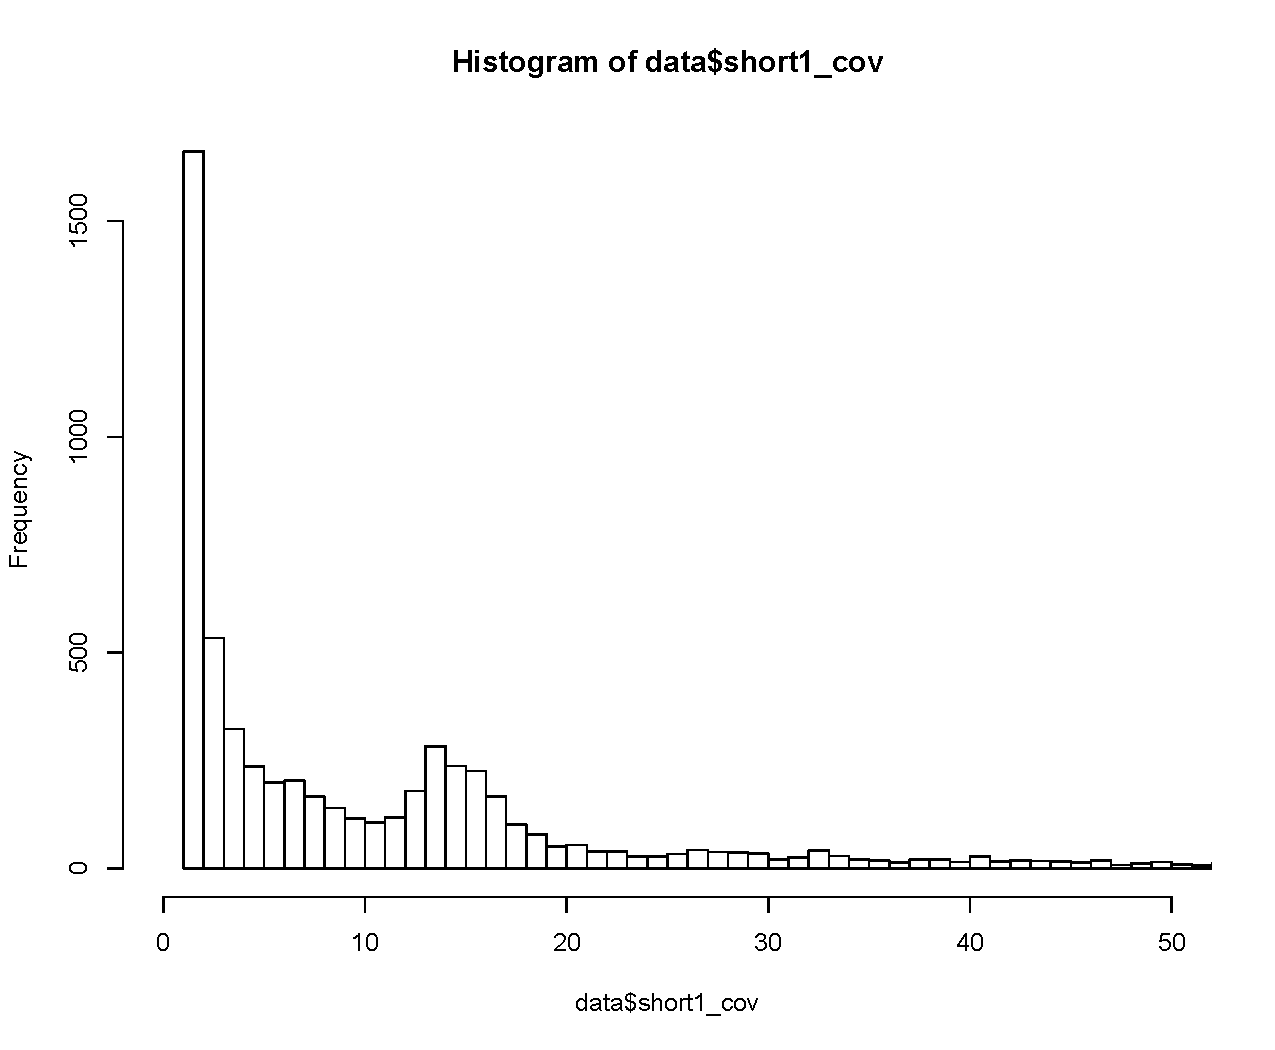
\includegraphics[keepaspectratio=true,width=300bp]{./Suis_plot_1.pdf}

However, if you weight the results with the node lengths (you need to install the \emph{plotrix} package for R to do this):
\begin{verbatim}
(R) > library(plotrix)
(R) > weighted.hist(data$short1_cov, data$lgth, breaks=0:50)
\end{verbatim}
\ldots you obtain:

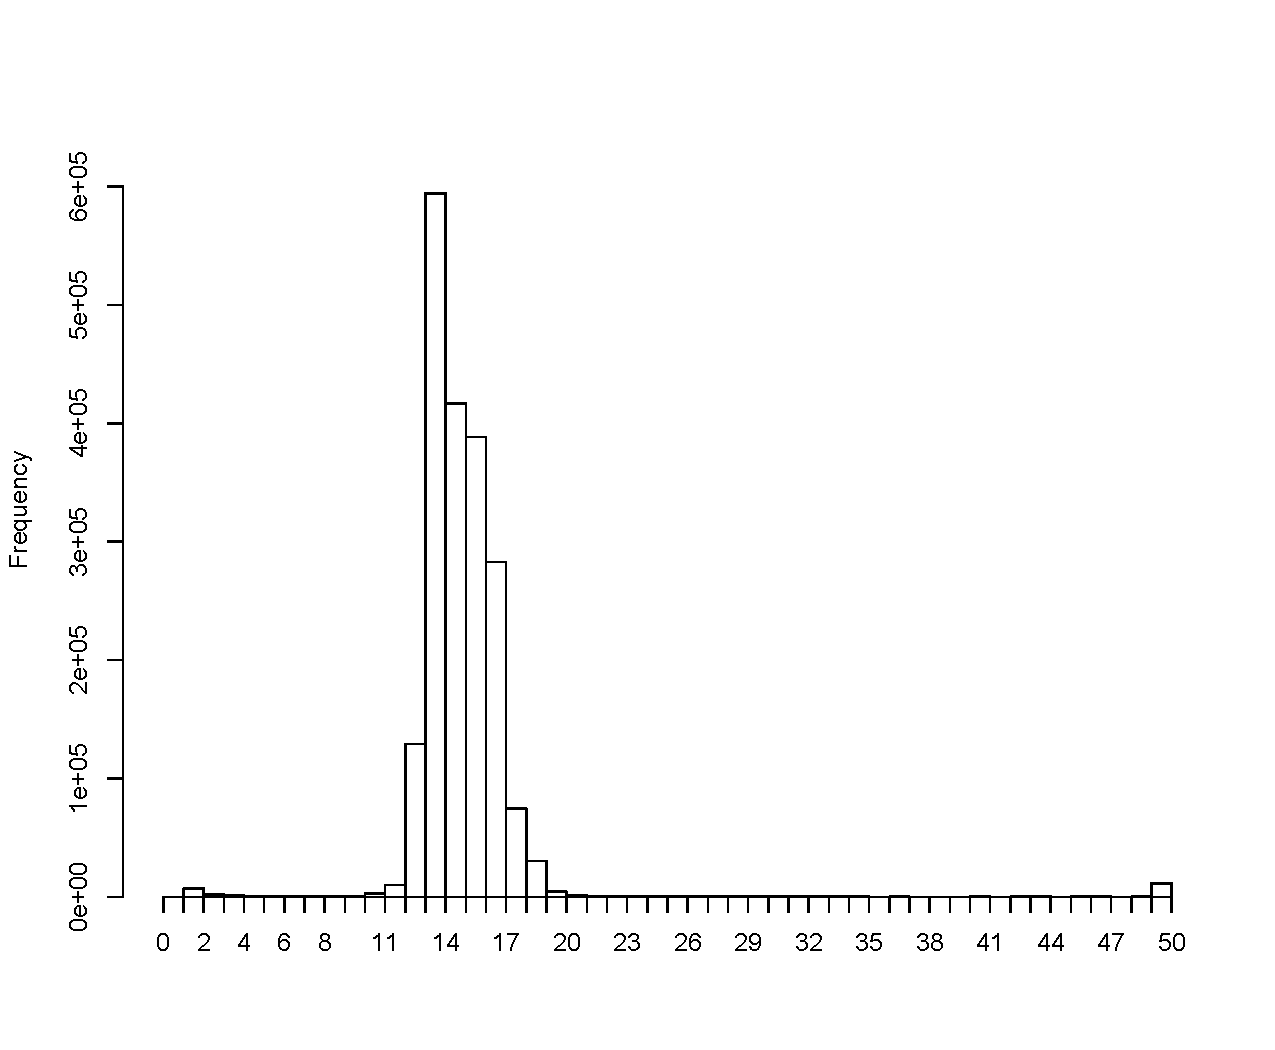
\includegraphics[keepaspectratio=true,width=300bp]{./suis_plot.pdf}

The comparison of these two plots should convince you that below 7 or 8x you find mainly short, low coverage nodes, which are likely to be errors. Set the exact cutoff at your discretion.

However beware that there is such a thing as an over-aggressive cutoff, which could create mis-assemblies, and destroy lots of useful data.

If you have read-pair information, or long reads, it may be profitable to set a low coverage cutoff and to use the supplementary information resolve the more ambiguous cases.

\subsection{Determining the expected coverage}

\label{sec:expcov}

From the previous weighted histogram it must be pretty clear that the expected coverage of contigs is near 14x. 

\subsection{Visualising contigs and assemblies}

This section will be quite vague, as there are a number of solutions currently available, and presumably new ones under development. The following indications are just hints, as I have not done any exhaustive shopping nor benchmarking.

Most assembly viewers require an assembly format, which come in a variety of shapes and colours: ACE, AMOS, CELERA, TIGR, etc. Velvet only ouputs AMOS .afg files, but these can easily be converted with open-source software (\href{http://amos.sourceforge.net}{amos.sourceforge.net}).

\subsection{What's long and what's short?}

Velvet was pretty much designed with micro-reads (e.g. Illumina) as short and short to long reads (e.g. 454 and capillary) as long. Reference sequences can also be thrown in as long.

That being said, there is no necessary distinction between the types of reads. The only constraint is that a short read be shorter than 32kb. The real difference is the amount of data Velvet keeps on each read. Short reads are presumably too short to resolve many repeats, so only a minimal amount of information is kept. On the contrary, long reads are tracked in detail through the graph.

This means that whatever you call your reads, you should be able to obtain the same initial assembly. The differences will appear as you are trying to resolve repeats, as long reads can be followed through the graph. On the other hand, long reads cost more memory. It is therefore perfectly fine to store Sanger reads as ``short'' if necessary.

\section{Contributed software}

The Velvet package is bundled with programs developed by other programers which could be useful to Velvet users:

\begin{description}
\item[afg\_handling] by Simon Gladman (Simon.Gladman@csiro.au)

These two scripts allow you to examine the (generally) large .afg files which can be produced by Velvet:

\begin{description}
 
\item[asmbly\_splitter] allows you to choose a specific scaffold from the assembly and produce a self-standing .afg file for that scaffold.

\item[snp\_view] produces an ASCII pileup display of the reads above a given locus 

\end{description}

\item[layout] by Paul Harrison (pfh@logarithmic.net)

This script converts a (Last)Graph file into a .dot file, which can then be converted into an image by GraphViz (www.graphviz.org). This allows you to directly observe the topology of a graph.

\item[VelvetOptimiser] by Simon Gladman (Simon.Gladman@csiro.au)

This script automatically finds the optimal parameter settings for Velvet.

\item[estimate-exp\_cov] by Torsten Seeman (torsten.seemann@infotech.monash.edu.au)

This script automatically determines the expected coverage value as described in the manual, and displays an ASCII histogram, thus obviating the need to start R for each Velvet run.

\item[fasta2agp] by David Studholme (david.studholme@tsl.ac.uk )

This script converts a Velvet assembly in FastA format with N's in the gaps 
into a AGP file which can be submitted to the EMBL or the NCBI.

\item[extractContigReads] by Daniel Zerbino (zerbino@ebi.ac.uk), suggested by Jasper Rees

This script scans the Graph2 file produced by Velvet and produces a FastA file
of all the reads which belong to a given contig.

\item[observed-insert-lengths] by Daniel Zerbino

This scripts scans the Graph2 file produced by velvetg then computes and displays the insert length distribution of a chosen short read library in the assembly.

\item[shuffleSequences] by Eric Cabot (ecabot@wisc.edu) Peter (peter@maubp.freeserve.co.uk) and Daniel Zerbino (zerbino@ebi.ac.uk)

Alternative ways to efficiently shuffle your reads produced in the language of your choice: C, BioPython, Perl or Bash.

\item[show\_repeats] by Ken Doig (kdd@doig.org)

Plots out the length of the larger repeated contigs in the assembly.

\item[AssemblyAssembler] by Jacob Crawford (jc598@cornell.edu)

Tries out different values of k, then merges all the different assemblies into
one.

\end{description}

\section{For more information}

\paragraph{Publication:}
 
 \label{sec:paper}
 
For more information on the theory behind Velvet, you can turn to:
\begin{quote}
D.R. Zerbino and E. Birney. 2008. Velvet: algorithms for de novo short read assembly using de Bruijn graphs. \emph{Genome Research}, \textbf{18}: 821-829
\end{quote}
Please use the above reference when citing Velvet.

\paragraph{Webpage:}

For general information and FAQ, you can first take a look at 
\href{http://www.ebi.ac.uk/~zerbino/velvet/}{www.ebi.ac.uk/$\sim$zerbino/velvet}.

\paragraph{Mailing list:}

For questions/requests/etc. you can subscribe to the users' mailing list: velvet-users@ebi.ac.uk.

To do so, see \href{http://listserver.ebi.ac.uk/mailman/listinfo/velvet-users}{listserver.ebi.ac.uk/mailman/listinfo/velvet-users} .


\paragraph{Contact emails:}

For specific questions/requests you can contact us at the following addresses:
\begin{itemize}
\item Daniel Zerbino $<$\href{mailto:zerbino@ebi.ac.uk}{zerbino@ebi.ac.uk}$>$
\item Ewan Birney: $<$\href{mailto:birney@ebi.ac.uk}{birney@ebi.ac.uk}$>$
\end{itemize}

\paragraph{Reporting bugs:}

We are very grateful to all the people who send us bugs. However, to speed up the process and avoid useless delays, please:
\begin{enumerate}
\item ensure that you have the very last version of Velvet, to the last digit, as displayed on the \href{http://www.ebi.ac.uk/~zerbino/velvet/}{website}.
\item attach to your e-mail the Log file from within the Velvet directory.
\item if the program crashed and created a core dump file could you please:
\begin{enumerate}
\item destroy the core.* file
\item recompile Velvet with the instruction ``make debug''
\item re-run Velvet and let it crash (therefore creating a new core file)
\item launch the GNU debugger with the instructions:
\begin{verbatim}
> gdb ./velvetg core.*
\end{verbatim}
\item within gdb, request a backtrace:
\begin{verbatim}
(gdb) bt full
\end{verbatim}
\item send the listing with the entire gdb session.
\end{enumerate}
\end{enumerate}

\end{document}
